\section{Theoretische Vorbereitung}
    \subsection{Grundlegende Beziehungen}
        \subsubsection{Magnetfelder}
            Die magnetische Flussdichte $\vec{B}$ ist ein Vektorfeld, das im SI-System die Einheit Tesla hat.
            Das $\vec{B}$ - Feld ist jedoch keine direkt messbare Gr"o"se, die zugeh"orige Messgr"ose ist die magnetische Feldst"arke $\vec{H}$.
            Diese wird in Ampere pro Meter angegeben ($\frac{A}{m}$) und ist im Vakuum direkt proportional
            zum $\vec{B}$ - Feld. Dort gilt:
            \begin{equation}
                \vec{B} = \mu_0 \vec{H}
            \end{equation}
            $\mu_0 = 4\pi \cdot 10^{-7}\frac{N}{A^2}$ bezeichnet dabei die magnetische Permeabilit"at des Vakuums.
            In Anwesenheit eines Materials mit der Magnetisierung $\vec{M} [\frac{A}{m}]$, welche die r"aumliche Dichte der im Material induzierten oder permanenten magnetischen Dipolmomente $\vec{\mu}$ angibt ($\vec{M} = \frac{d\vec{\mu}}{dV}$), "andert sich der Zusammenhang zu
            \begin{equation}
                \vec{B} = \mu_0 (\vec{H} + \vec{M})
            \end{equation}
            Zus"atzlich l"asst sich die magnetische Suszeptibilit"at $\chi$ nutzen, um beispielsweise die Relation zwischen $\vec{H}$ und $\vec{M}$ zu beschreiben:
            \begin{equation}
                \vec{M} = \chi \vec{H}
            \end{equation}
            Die magnetische Suszeptibilit"at beschreibt dabei, wie stark sich die Magnetisierung in einem
            Material, das sich in einem externen Magnetfeld befindet, "andert, bzw. wie viele der magnetischen Momente sich entlang des externen Feldes ausrichten.
            Dabei Unterscheidet man im Allgemeinen zwischen
            \begin{itemize}
                \item $\chi > 0$ Paramagneten
                \item $\chi < 0$ Diamagneten
            \end{itemize}
            Daraus ergibt sich "uber
            \begin{equation}
                \mu = \mu_0 (1 + \chi)
            \end{equation}
            die magnetische Permeabilit"at $\mu [\frac{N}{A^2}]$, die das Verh"altnis zwischen magnetischer Flussdichte $B$ und magnetischer Feldst"arke $H$ beschreibt:
            $$ \mu = \frac{B}{H}$$
            Das magnetische (Dipol-)Moment $\vec{\mu}$ [$\frac{A}{m^2}$] ist ein Ma"s f"ur die St"arke
            und Richtung eines magnetischen Dipols. Es l"asst sich jedoch auch f"ur Str"ome definieren, beispielsweise gilt f"ur eine ebene
            Leiterschleife (Strom $I$) mit Fl"ache $A$ und Fl"achennormalenvektor $\vec{n_A}$:
            \begin{equation}
                \vec{\mu} = A I \vec{n_A}
            \end{equation}
            In einem externen $\vec{B}$ - Feld wirkt auf einen magnetischen Dipol $\vec{\mu}$ ein Drehmoment $\vec{D}$:
            \begin{equation}
                \vec{D} = \vec{\mu} \times \vec{B}
            \end{equation}.
            Erweitert man das Konzept einer Leiterschleife zu einer Reihe von Leiterschleifen, erh"alt man das Magnetfeld einer Spule der L"ange $l$ mit $N$ Windungen, durch die ein Strom $I$ flie"st:
            \begin{equation}
                B = N \frac{\mu_0 I}{l}
            \end{equation}
    \subsection{Magnetismus ohne Ordnungsph"anomene}
        \subsubsection*{gyromagnetisches Verh"altnis}
            Das gyromagnetische Verh"altnis $\gamma$ eines magnetischen Moments $\mu$ wird beschrieben "uber das Verh"altnis
            des magn. Moments zu dessen Drehimpuls $L$:
            \begin{equation}
                \gamma = \frac{\mu}{L}
            \end{equation}
        \subsubsection*{Spin-,Bahnmagnetismus und Land\'e-Faktor}
            Alle Teilchen, die sowohl einen Drehmoment $\vec{\ell}$ als auch eine elektrische Ladung $q$ besitzten, haben ein magnetisches Dipolmoment $\vec{\mu_{\ell}}$:
            \begin{equation}
                \vec{\mu_{\ell}} = \frac{q}{2m} \vec{\ell}
            \end{equation}
            Dies wird allgemein als Bahnmagnetismus beschrieben. Analog dazu gilt eine "ahnliche formel f"ur den Spin $\vec{s}$:
            \begin{equation}
                \vec{\mu_s} = \frac{q\cdot g_s}{2m} \vec{s}
            \end{equation},
            bei dem der anomale Spin-$g$-Faktor zu ber"ucksichtigen ist.
            Das Bohr'sche Magneton $\mu_B$ ist der Betrag des magnetischen Moments, welches ein Elektron
            mit $\ell=1$ erzeugt, also im Grundzustand:
            \begin{equation}
                \mu_B = \frac{e \hbar}{2 m_e} = 5,7883818060(17)\cdot 10^{-5} \frac{eV}{T}
            \end{equation}
            Das magnetische Moment eines Elektrons wird meist durch ein Vielfaches des Bohr'schen
            Magnetons beschrieben.
            Der Land\'e-Faktor ist das Verh"altnis der Diskrepanz zwischen gemessenem magnetischen Moment
            und dem \dq klassisch\dq errechneten eines Elektrons. F"ur Elektronen ist $g_s \approx 2$.
        \subsubsection*{Diamagnetismus}
            Bei einem Diamagneten richten sich die inneren magnetischen Momente entgegengesetzt
            zu einem "au"seren Magnetfeld aus. Dies passiert aufgrund der unten erkl"arten Lenz'schen Regel.
            Au"serhalb eines magnetischen Feldes sind Diamagneten
            nicht magnetisiert. Der einzige ideale Diamagnet ist ein Supraleiter, bei denen gilt $\chi = -1$
        \subsubsection*{Lenz'sche Regel}
            Die Lenz'sche Regel besagt, dass eine "Anderung eines Magnetfeldes $\vec{B}$ einen der "Anderung
            entgegenwirkenden Strom induziert, vgl. Abb. \ref{figLenz}.

            \begin{figure}[H]
                \centering
                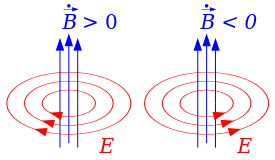
\includegraphics{Images/lenzRegel.png}
                \label{figLenz}
                % https://de.wikipedia.org/wiki/Datei:Electromagnetic_induction.svg
            \end{figure}
        \subsubsection*{Langevin-Gleichung}
        Die Larmor-Frequenz $\omega_L$ des Elektrons ist gegeben "uber $\omega_L = |\gamma | B$, mit $\gamma = -\frac{e}{2m_e}$, woraus sich $\omega_L = \frac{eB}{2m_e}$ ergibt. Daraus ergibt sich f"ur $Z$ Elektronen ein durch die Larmor-Pr"azession hervorgerufener Strom $I$:
        \begin{equation}
        	I = Q \cdot f
        \end{equation}
        Dabei ist $Q = -Ze$ und die Frequenz $f = \frac{\omega_L}{2\pi}$:
        \begin{equation}
        	I = \frac{Ze^2 B}{4\pi m_e}
        \end{equation}
Daraus resultiert wiederum ein magnetisches Moment $\mu = I \cdot A$ (vgl. ebene Leiterschleife), wobei f"ur die Fl"ache $A = \pi \langle \rho^2 \rangle$, mit dem mittleren quadratischen Abstand der Elektronen vom Kern $\langle \rho^2 \rangle$, angesetzt werden kann.\\
Nutzt man nun noch aus, dass $\langle \rho^2 \rangle = \langle x^2 \rangle + \langle y^2 \rangle$ und $\langle r^2 \rangle = \langle x^2 \rangle + \langle y^2 \rangle + \langle z2 \rangle$, so kann $\langle \rho^2 \rangle$ ersetzt werden durch $\frac{2}{3} \langle r^2 \rangle$. F"ur $N$ Atome pro Einheitsvolumen ergibt sich mit diesen "uberlegungen f"ur deren magnetische Suszeptibilit"at $\chi = \frac{N\mu}{B}$ die Langevin - Gleichung:
	\begin{equation}
		\chi = - \frac{NZe^2}{6m_e} \langle r^2 \rangle
	\end{equation}
        \subsubsection*{Paramagnetismus}
            Ein Paramagnet besitzt eine positive Suszeptibilit"at, ist jedoch ohne "au"seres
            Magnetfeld nicht magnetisiert. In einem Paramagneten richten sich die inneren magnetischen Momente
            in Feldrichtung aus.
            \subsubsection*{Einzelbeitr"age}
            Der Pauli-Paramagnetismus entsteht durch freie Elektronen in Metallen, die "uber ihren Spin
            ein magnetisches Moment besitzen. Da jedoch, aufgrund des Pauli-Prinzips, nur angeregte
            Leitungselektronen mit Energie oberhalb der Fermi-Energie sich nach dem Magnetfeld ausrichten k"onnen,
            ist die Anzahl der beitragenden Elektronen proportional zur Materialabh"angigen Fermi-Temperatur:
            \begin{equation}
                \chi_{Pauli} \thicksim \frac{C}{T} \cdot \frac{T}{T_{F}} = \frac{C}{T_F}\thicksim 10^{-6 ... -5}
            \end{equation}
            mit der Curie-Konstante $C$, der Temperatur $T$ und der Fermi-Temperatur $T_F$.
            \\
            Die gitterbildenden Atome k"onnen ebenfalls zum Paramagnetismus beitragen. Dies geschieht immer dann, wenn diese Atome nicht vollst"andig gef"ullte Schalen und somit ein verbleibendes magnetisches Moment haben. Der dadurch hervorgerufene sogenannte atomare bzw. Langevin - Paramagnetismus ist $T$ - abh"angig und liefert einen st"arkeren Beitrag zum Gesamtmagnetismus als die Leitungselektronen:
            \begin{equation}
            	\chi_{Langevin} \thicksim \frac{C}{T} \thicksim 10^{-3 ... -2}
            \end{equation}
			Dieser Effekt kann auch dann auftreten, wenn die Schalen der gitterbildenden Atome komplett gef"ullt sind, da durch thermische Anregungen stets einige dieser Atome in angeregten Zust"anden sind, in welchen der Gesamtdrehimpuls und folglich das magnetische Moment trotzdem ungleich Null sind. In diesem Fall spricht man von Van - Fleck - Paramagnetismus, dessen Beitrag sich in "ahnlichen Gr"o"senordnungen bewegt, wie der Pauli - Paramagnetismus:
			\begin{equation}
				\chi_{Van - Fleck} \thicksim 10^{-6 ... -5}
			\end{equation}
			


    \subsection{Magnetismus mit Ordnung}
        \subsubsection*{Wechselwirkung}
            Die Magnetische Ordnung kommt zustande "uber die sogennante Austauschwechselwirkung, bei welcher sich
            die atomaren Gesamtdrehmomente ein energietisches Minimum erstrebend zueinander Ausrichten. Dabei ist
            das Pauli-Prinzip ein entscheidener Faktor, da durch dieses bei Fermionen viele der "uberg"ange verboten sind.
            Ein h"aufig verwendetes Modell zur Beschreibung dieser Austauschwechselwirkung ist das Ising-Modell.
        \subsubsection*{Anisotropie}
            Magnetisch leichte Achsen bzw Schwere Achsen beschreiben Achsen entlang denen die Magnetisierung bevorzugt
            bzw. nur unter gro"sem Aufwand stattfindet. Die Anisotropieenergie bezeichnet dabei die notwendige Energie
            um eine Magnetisierung von einer leichten in eine schwere Achse zu drehen.\\
            Anisotropieenergie spaltet sich dabei grob in 3 Terme auf:
            \begin{itemize}
                \item \textbf{Magnetokristalline Anisotropie}, hervorgerufen durch die Anisotropie einer Kristallstruktur
                \item \textbf{Formanisotropie}, resultierend aus der Probengeometrie
                \item \textbf{induzierte Anisotropie}, durch Spannungen aufgrund von Unregelm"a"sigkeiten.
            \end{itemize}
        \subsubsection*{Ferro-, Ferri-, Antiferromagnetismus}
            Ferromagneten Zeichnen sich dar"uber aus, dass sich sog. Weiss'sche Bezirke bilden. In diesen Bezirken
            kommt es zu einer spontanten Magnetisierung der magn. Dipole. Das bedeutet, dass sich die Dipole entlang einer
            gemeinsamen Vorzugsrichtung ausrichten. Dieses Verhalten kann spontan und unabh"angig von einem "ausseren Magnetfeld
            auftreten, wird es jedoch durch ein solches induziert bleibt es im Anschluss auch in Abwesehnheit eines solchen bestehen.
            Beim Ferrimagnetismuss verh"alt es sich recht Analog, jedoch sind einige Dipole entgegengesetzt ausgerichtet.
            Dabei kommt es jedoch nicht zu einer Aufhebung der Gesamtmagnetisierung, da in ferrimagnetischen Materialen
            eine Ausrichtung bevorzugt, d.h. st"arker ist, wodurch eine Gesamtmagnetisierung entsteht.
            Bei antiferromagnetischen Materialen verh"alt es sich wie bei Ferrimagnetischen Materialen ohne Vorzugsrichtung,
            wodurch sich insgesamt keine Magnetisierung durchsetzt, es bleibt unmagnetisch.
            \begin{figure}[H]
                \centering
                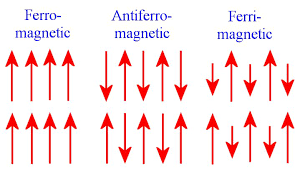
\includegraphics{Images/ferroferrianti.png}
            \end{figure}
        \subsubsection*{Ferromagnetismus}
            Wie bereits angesprochen kommt es in ferromagnetischen Materialien zu sog. Weiss'schen Bezirken,
            oder auch Dom"anen, die sich aufgrund der Kristallstruktur und dessen inhomogenit"aten ausbilden. Dabei
            h"angt die Vorzugsrichtung des jeweiligen Bezirks vom Kristallgitter der Probe ab. Solche
            Bezirke erstrecken sich von etwa 10 bis 1000$\mu m$ in linearer Ausdehnung.\\
            An den "uberg"angen von zwei Weiss'schen Bezirken bilden sich Bloch-W"ande, in denen die magnetischen Momente st"uckweise von den Ausrichtungen innerhalb der angrenzenden Weiss-Bezirke ineinander "ubergehen.\\
            In Anwesenheit eines externen Feldes verschieben sich diese Bloch-W"ande nun zugunsten einer Ausrichtung der magnetischen Momente entlang des externen Feldes. Wird die externe Feldst"arke erh"oht, kann es dabei zu Barkhausenspr"ungen kommen, bei welchen sich komplette Weissbezirke spontan ummagnetisieren. Diese Ummagnetisierungen sind stets reversibel, indem man die Richtung des externen Magnetfelds umkehrt. Dabei treten Hysterese-Effekte auf, die wir im Folgenden beschreiben.
           % \hl{todo: Energie, Wandversch., Drehung, Barkhausenspruengen, Reversibilitaet}
        \subsubsection*{Hysteresekurve}
            Hysteresekurven treten in vielen Bereichen der Physik auf, in diesem Fall wird jedoch die Magnetisierung
            der Probe in Abh"angigkeit eines "ausseren Feldes aufgetragen.\\
            F"uhrt man eine Solche Messung durch, beginnt der Graph mit der sogennanten Neukurve, dabei richten sich
            die Weiss'schen Bezirke das erste mal aus bis zum Punkt der S"attigung. Misst man dann die Magnetisierung bei einem Abnehmenden Magnetfeld
            kommt man zun"achst zum Remanenzfeld, welches bestehenbleibt obwohl kein "ausseres Feld mehr angelegt ist. Wird die externe Feldst"arke nun entgegen der anf"anglichen Ausrichtung erh"oht, nimmt die Restmagnetisierung weiter ab, bis
            sie beim Erreichen des Koerzitivfeldes schlie"slich verschwindet und es erneut zur spontanen Magnetisierung kommt und der Vorgang von neuem Beginnt.
            \begin{figure}[H]
                \centering
                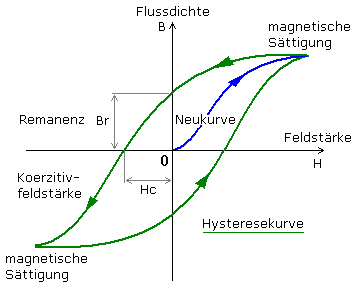
\includegraphics[width=0.9\textwidth]{Images/hyster.png}
                %https://www.google.com/url?sa=i&url=https%3A%2F%2Fwww.elektroniktutor.de%2Felektrophysik%2Fmagkurve.html&psig=AOvVaw202TVqiaXyCzzC35HNuQiG&ust=1622981447740000&source=images&cd=vfe&ved=0CAMQjB1qFwoTCLi505e7gPECFQAAAAAdAAAAABAD
            \end{figure}

%            Zeigen Sie, dass der Fl"acheninhalt der Hysteresekurve ein Ma"s fur die Energie ist, die beim einmaligen Umfahren der Kurve als W"arme
%            auftritt (Verlust).
            Je h"oher die Energie ist, die aufgebracht werden muss um die Weiss'schen Bezirke auszurichten, desto gr"o"ser ist die
            Remanenz und die Koerzitivfeldst"arke. Und je gr"o"ser Remanenz und Koerzitivfeldst"arke, desto gr"o"ser die Fl"ache unter der Hysteresekurve.
            Der Fl"acheninhalt der Hysteresekurve ist also proportional zur ben"otigten Energie, die f"ur ein einmaliges Umfahren der Kurve ben"otigt wird.
            
        \subsubsection*{magn. Hart und Weich}
            Magnetisch weiche Stoffe zeichen sich durch eine besonders leichte Magnetisierbarkeit aus. Das bedeutet,
            dass sie ein kleineres Koerzitivfeld haben. Harte
            magnetische Stoffe sind hingegen nur schwer magnetisierbar.
            \begin{figure}[H]
                \centering
                \includegraphics[width=0.9\textwidth]{Images/"ubersicht_Koerzitivfeldst"arke.png}
                %https://de.wikipedia.org/wiki/Magnetwerkstoffe#/media/Datei:%C3%9Cbersicht_Koerzitivfeldst%C3%A4rke.svg
            \end{figure}
        \subsubsection*{Ferrite}

        \subsubsection*{Temperatureinfluss}
            Bei steigenden Temperaturen f"uhrt die thermische Energie zu Bewegung im Material, wodurch die Ordnung der
            Dipole gest"ort wird. Je h"oher die Temperatur ist, desto schwieriger wird es f"ur die Dipole, ihre Ausrichtung entlang
            der Feldlinien beizubehalten. Steigt die Temperatur "uber die sog. Curie Temperatur, verliert das Material g"nzlich
            die Eigenschaft der magnetischen Ausrichtung und wird nichtmagnetisch.
        \subsubsection*{Phasen"ubergang}
            %https://sci-hub.se/https://link.springer.com/chapter/10.1007/978-3-642-82138-7_1
<<<<<<< Updated upstream
            Bei Thermondynamischen Phasen"uberg"ange spricht man h"aufig "uber eine Spontane "anderung der Freien Energie F.
            Bei ihnen wird zwischen "uberg"angen erster und zweiter Ordnung Unterschieden. "uberg"ange erster Ordnung
            arbeiten mit latenter W"arme, also ohne Temperatur"anderung. Dabei tauscht das System eine Feste menge an energy
=======
            Von Thermondynamischen Phasen"uberg"angen spricht man dann, wenn eine spontane "Anderung der Freien Energie $F$ auftritt.
            Dabei unterscheidet man zwischen "Uberg"angen erster und zweiter Ordnung. "Uberg"ange erster Ordnung
            arbeiten mit latenter W"arme, also ohne Temperatur"anderung. Dabei tauscht das System eine feste Menge an Energie
>>>>>>> Stashed changes
            mit der Umgebung aus.\\
            Bei "Uberg"angen zweiter Ordnung ist keine solche Spontanit"at zu erkennen, sie werden daher auch als kontinuierliche Phasen"uberg"ange bezeichnet. Man definiert einen Phasen"ubergang $n$-ter Ordnung allgemein "uber die freie Enthalpie $G$: sind $G$ und die ersten $n-1$ Ableitungen von $G$ nach ihren freien Variablen stetig, die $n$-ten Ableitungen jedoch unstetig am Phasen"ubergang, so handelt es sich um einen "Ubergang $n$-ter Ordnung.
            \begin{figure}[H]
                %https://en.wikipedia.org/wiki/Phase_transition
                \centering
                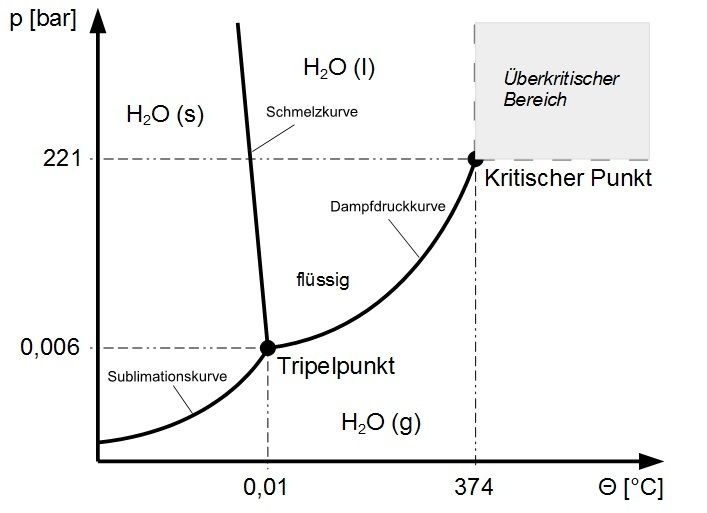
\includegraphics[width=0.9\textwidth]{Images/waterphase.jpg}
            \end{figure}
    \subsection{Entmagnetisierungsfaktor}

        \subsubsection*{Entmagnetisierung}
<<<<<<< Updated upstream
            Eine Entmagnetisierung ist ein Vorgang, indem das Magnetfeld eines Magneten verschwindet.
            Die Ursache hierf"ur k"onnen: Ersch"utterung, Hitze sein. Aber meist wird ein Material
            durch ein zuerst starkes Wechsel-Magnetfeld, welches aber mit der Zeit abklingt, verwendet.
=======
    		Entmagnetisierung ist der Vorgang, bei dem das Magnetfeld eines Magneten dauerhaft verschwindet.
            Die Ursache hierf"ur k"onnen Ersch"utterungen, Hitze oder - f"ur ferro- bzw ferrimagnetische Materialien - das Koerzitivfeld sein: Bringt man ein solches Material
            in ein zuerst starkes Wechsel-Magnetfeld, welches aber mit der Zeit abklingt, kann es gezielt entmagnetisiert werden.
            \hl{Bild}
>>>>>>> Stashed changes
            \begin{figure}[H]
                \centering
                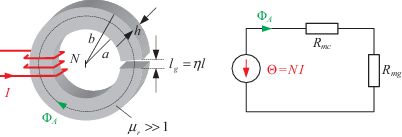
\includegraphics{images/Ringkern}
            \end{figure}
        \subsubsection*{Herleitung Entmagnetisierungsfaktors}
            Man nimmt an, dass die L"ucke des Rings sehr klein ist und die Feldlinien sich homogen
            fortsetzen. Dann vergleicht man die Erregerfelder mit und ohne Luftspalt. Dies geht, da
            bei beiden die gleiche Stromst"arke verwendet wird.
            \begin{equation}
                H \cdot L = H_R \cdot L_R + H_L \cdot L_L
            \end{equation}
            Dabei ist $L = 2 \pi r$ der Umfang des Kerns und $L_L, L_R$ sind die L"ange der L"ucke bzw. des restlichen Kerns.
            $H_R, H_L$ sind die Erregerfelder im Ring und in der L"ucke.
            Mit den Maxwellgleichungen und dem Stokes'schen Satz folgt:
            \begin{equation}
                B_R \cdot F = B_L \cdot F
            \end{equation}
            hier ist $F$ die Querschnittsfl"ache des Rings. Es gilt allgemein:
            \begin{equation}
                B = \mu_0 (H + M)
            \end{equation}
            Da Luft als Vakuum gen"ahert werden kann, ist $M=0$ in der L"ucke.
            Durch diese Gleichungen ergeben sich f"ur $H_R$ bzw. $H_L$:
            \begin{align*}
                H_R = H - \frac{L_L}{L} M\\
                H_L = H + \frac{L_L}{L} M
            \end{align*}
            Das entmagnetisierende Feld ist damit:
            \begin{equation}
                H_e = \frac{L_L}{L} M
            \end{equation}
            mit dem Entmagnetisierungsfaktor $N = \frac{L_L}{L}$
        \subsubsection*{gescherte Hysteresenkurven}
            %https://www.google.com/url?sa=i&url=https%3A%2F%2Fsilo.tips%2Fdownload%2Fmagnetisierungskurven-eines-ferrits-1&psig=AOvVaw1-iHGdJClryjKD8ByJthm3&ust=1623062593991000&source=images&cd=vfe&ved=0CAIQjRxqFwoTCMjA4MHpgvECFQAAAAAdAAAAABAO
            Da bei steigender Spaltbreite das entmagnetisierende Feld $H_{ent}$ immer gr"o"ser wird, werden wir das erzeugende Feld $H_{ohne}$
            auch steigern m"ussen. Wenn man in einem M-H-Diagramm eine Hysterese f"ur einen Ringkern
            ohne Luftspalt aufnimmt, so ist $H_{E}=H_{ohne}$. F"ur Hyteresen mit Ringkernen,
            die einen Luftspalt besitzen, steigen die $H_{ohne}$-Werte, die die gleiche Magnetisierung
            bzw. das gleiche $H_{E}$ erzeugen, immer weiter an, sodass die Hysterese nach rechts
            geschert wird. Man nennt diese Hysteresen daher auch gescherte Hysteresen.
            \begin{figure}
                \centering
                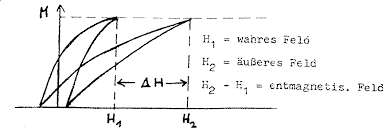
\includegraphics[width=0.9\textwidth]{Images/geschert.png}
            \end{figure}

        \subsubsection*{Einfluss der Entmagnetisierung auf $\chi$}
            Die sog. scheinbare Suszeptibilit"at $\chi_s$ l"asst sich definieren "uber
            \begin{equation}
                \chi_s = \frac{M}{H_{ohne}}
            \end{equation}
            Die wahre Suszeptibilit"at $\chi_w$ l"asst sich "uber das effektive Feld definieren als
            \begin{equation}
                \chi_w = \frac{M}{H_{E}}
            \end{equation}
            Nutzt man nun die Beziehung zwischen dem effektiven Feld und dem Feld ohne Material
            \begin{equation}
                H_E = H_{ohne} - N\cdot M
            \end{equation}
            folgt damit
            \begin{equation}
                \frac{M}{\chi_w} = \frac{M}{\chi_s} - N \cdot M
            \end{equation}
            \begin{equation}
                \chi_s = \frac{\chi_w}{1+N\cdot \chi_w}
            \end{equation}
